\begin{figure}[htpb]
\centering
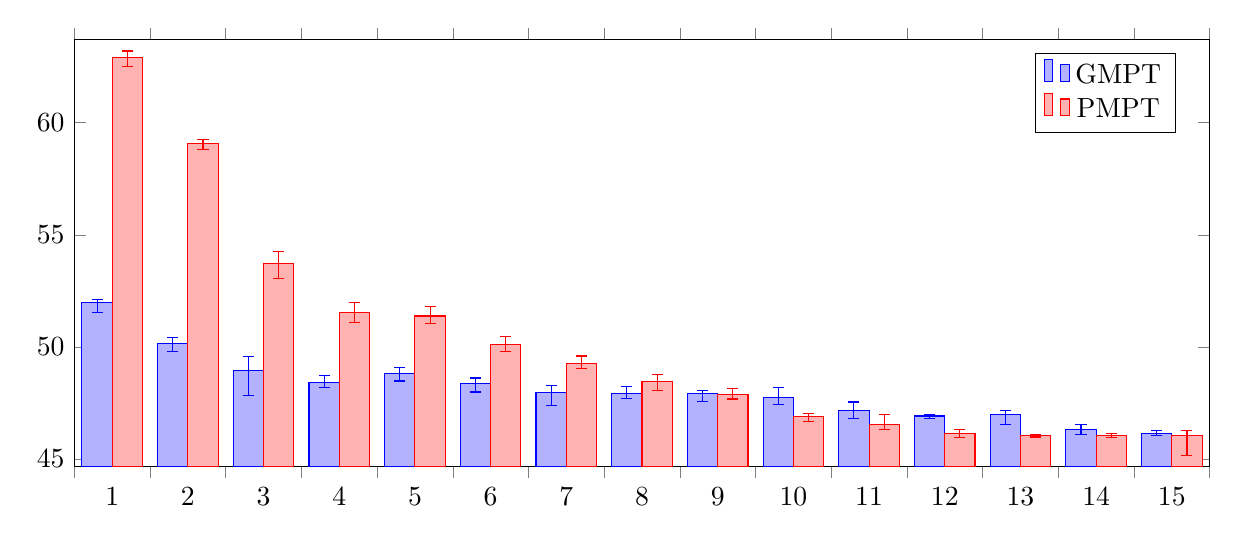
\begin{tikzpicture}
\begin{axis}[
legend pos=north east,
enlargelimits={abs=0.5},
ybar=0pt,
bar width=0.4,
width=16cm,
height=7cm,
xtick={0.5,1.5,...,15.5},
xticklabels={1,...,15},
x tick label as interval
]

\addplot+[error bars/.cd,
y dir=both,y explicit]
coordinates {
    (1,51.9717888360177) += (0,0.141352491928259) -= (0,0.440010384184291)
    (2,50.1668987014317) += (0,0.238370750062352) -= (0,0.383128825312589)
    (3,48.9597483322356) += (0,0.595847508010500) -= (0,1.13150258988060 )
    (4,48.4231287588079) += (0,0.311258328716740) -= (0,0.236621447616535)
    (5,48.8076411054881) += (0,0.285988081180335) -= (0,0.326400991856147)
    (6,48.3728427696685) += (0,0.244936635861023) -= (0,0.383344786044226)
    (7,47.9826060171152) += (0,0.316025495323878) -= (0,0.591076671783732)
    (8,47.9107471809450) += (0,0.333779739462024) -= (0,0.215802033233381)
    (9,47.9206716243684) += (0,0.145610298716868) -= (0,0.358475598043476)
    (10,47.7339920728808) += (0,0.470780310921576) -= (0,0.284585375560390)
    (11,47.1496451599979) += (0,0.396135675248004) -= (0,0.356532442258683)
    (12,46.9225169858525) += (0,0.083227037504123) -= (0,0.114008695210025)
    (13,46.9903069318091) += (0,0.165056482525436) -= (0,0.445691370610206)
    (14,46.3225907340171) += (0,0.229486697802720) -= (0,0.214732313990730)
    (15,46.1342095502068) += (0,0.156640264836348) -= (0,0.093178147706538)};
\addplot+[error bars/.cd,
y dir=both,y explicit]
coordinates {
    (1,62.9278466811292) += (0,0.271521963473894) -= (0,0.427830872232605)
    (2,59.0598958757091) += (0,0.184168050399308) -= (0,0.255963530411819)
    (3,53.7337342397985) += (0,0.525729721145588) -= (0,0.687987842917067)
    (4,51.5474633980814) += (0,0.445812278746146) -= (0,0.467156937429273)
    (5,51.3803222815890) += (0,0.421162669734969) -= (0,0.319064141418743)
    (6,50.1078772800408) += (0,0.345666170336202) -= (0,0.309568791318064)
    (7,49.2719090339404) += (0,0.325140846702602) -= (0,0.243064426806590)
    (8,48.4692716483709) += (0,0.316604304932078) -= (0,0.416873820104783)
    (9,47.8964031221703) += (0,0.232373753015530) -= (0,0.217349072849650)
    (10,46.8824137274556) += (0,0.161036214118710) -= (0,0.226334986945730)
    (11,46.5545351246186) += (0,0.447213228121889) -= (0,0.249776272179105)
    (12,46.1296161091866) += (0,0.208108546541233) -= (0,0.149696036370983)
    (13,46.0413393059249) += (0,0.039757343750920) -= (0,0.056483477251170)
    (14,46.0566087845517) += (0,0.075046329996077) -= (0,0.075049965010769)
    (15,46.0500422026862) += (0,0.226031183493483) -= (0,0.877295127739160)};
\legend{GMPT,PMPT}
\end{axis}
\end{tikzpicture}
\caption[Comparison GMPT PMPT]{Comparison\footnotemark of the temperature measurements for GMPT and PMPT}
\label{fig:i_eva_gpbar_n}
\end{figure}
\footnotetext{The bar values correspond to the median and the error bars correspond to the lower and upper inner fences displayed in the boxplots in \autoref{fig:i_eva_gp_n}}